% Options for packages loaded elsewhere
\PassOptionsToPackage{unicode}{hyperref}
\PassOptionsToPackage{hyphens}{url}
\PassOptionsToPackage{dvipsnames,svgnames,x11names}{xcolor}
%
\documentclass[
  letterpaper,
  DIV=11,
  numbers=noendperiod]{scrartcl}

\usepackage{amsmath,amssymb}
\usepackage{lmodern}
\usepackage{iftex}
\ifPDFTeX
  \usepackage[T1]{fontenc}
  \usepackage[utf8]{inputenc}
  \usepackage{textcomp} % provide euro and other symbols
\else % if luatex or xetex
  \usepackage{unicode-math}
  \defaultfontfeatures{Scale=MatchLowercase}
  \defaultfontfeatures[\rmfamily]{Ligatures=TeX,Scale=1}
\fi
% Use upquote if available, for straight quotes in verbatim environments
\IfFileExists{upquote.sty}{\usepackage{upquote}}{}
\IfFileExists{microtype.sty}{% use microtype if available
  \usepackage[]{microtype}
  \UseMicrotypeSet[protrusion]{basicmath} % disable protrusion for tt fonts
}{}
\makeatletter
\@ifundefined{KOMAClassName}{% if non-KOMA class
  \IfFileExists{parskip.sty}{%
    \usepackage{parskip}
  }{% else
    \setlength{\parindent}{0pt}
    \setlength{\parskip}{6pt plus 2pt minus 1pt}}
}{% if KOMA class
  \KOMAoptions{parskip=half}}
\makeatother
\usepackage{xcolor}
\setlength{\emergencystretch}{3em} % prevent overfull lines
\setcounter{secnumdepth}{5}
% Make \paragraph and \subparagraph free-standing
\ifx\paragraph\undefined\else
  \let\oldparagraph\paragraph
  \renewcommand{\paragraph}[1]{\oldparagraph{#1}\mbox{}}
\fi
\ifx\subparagraph\undefined\else
  \let\oldsubparagraph\subparagraph
  \renewcommand{\subparagraph}[1]{\oldsubparagraph{#1}\mbox{}}
\fi

\usepackage{color}
\usepackage{fancyvrb}
\newcommand{\VerbBar}{|}
\newcommand{\VERB}{\Verb[commandchars=\\\{\}]}
\DefineVerbatimEnvironment{Highlighting}{Verbatim}{commandchars=\\\{\}}
% Add ',fontsize=\small' for more characters per line
\usepackage{framed}
\definecolor{shadecolor}{RGB}{241,243,245}
\newenvironment{Shaded}{\begin{snugshade}}{\end{snugshade}}
\newcommand{\AlertTok}[1]{\textcolor[rgb]{0.68,0.00,0.00}{#1}}
\newcommand{\AnnotationTok}[1]{\textcolor[rgb]{0.37,0.37,0.37}{#1}}
\newcommand{\AttributeTok}[1]{\textcolor[rgb]{0.40,0.45,0.13}{#1}}
\newcommand{\BaseNTok}[1]{\textcolor[rgb]{0.68,0.00,0.00}{#1}}
\newcommand{\BuiltInTok}[1]{\textcolor[rgb]{0.00,0.23,0.31}{#1}}
\newcommand{\CharTok}[1]{\textcolor[rgb]{0.13,0.47,0.30}{#1}}
\newcommand{\CommentTok}[1]{\textcolor[rgb]{0.37,0.37,0.37}{#1}}
\newcommand{\CommentVarTok}[1]{\textcolor[rgb]{0.37,0.37,0.37}{\textit{#1}}}
\newcommand{\ConstantTok}[1]{\textcolor[rgb]{0.56,0.35,0.01}{#1}}
\newcommand{\ControlFlowTok}[1]{\textcolor[rgb]{0.00,0.23,0.31}{#1}}
\newcommand{\DataTypeTok}[1]{\textcolor[rgb]{0.68,0.00,0.00}{#1}}
\newcommand{\DecValTok}[1]{\textcolor[rgb]{0.68,0.00,0.00}{#1}}
\newcommand{\DocumentationTok}[1]{\textcolor[rgb]{0.37,0.37,0.37}{\textit{#1}}}
\newcommand{\ErrorTok}[1]{\textcolor[rgb]{0.68,0.00,0.00}{#1}}
\newcommand{\ExtensionTok}[1]{\textcolor[rgb]{0.00,0.23,0.31}{#1}}
\newcommand{\FloatTok}[1]{\textcolor[rgb]{0.68,0.00,0.00}{#1}}
\newcommand{\FunctionTok}[1]{\textcolor[rgb]{0.28,0.35,0.67}{#1}}
\newcommand{\ImportTok}[1]{\textcolor[rgb]{0.00,0.46,0.62}{#1}}
\newcommand{\InformationTok}[1]{\textcolor[rgb]{0.37,0.37,0.37}{#1}}
\newcommand{\KeywordTok}[1]{\textcolor[rgb]{0.00,0.23,0.31}{#1}}
\newcommand{\NormalTok}[1]{\textcolor[rgb]{0.00,0.23,0.31}{#1}}
\newcommand{\OperatorTok}[1]{\textcolor[rgb]{0.37,0.37,0.37}{#1}}
\newcommand{\OtherTok}[1]{\textcolor[rgb]{0.00,0.23,0.31}{#1}}
\newcommand{\PreprocessorTok}[1]{\textcolor[rgb]{0.68,0.00,0.00}{#1}}
\newcommand{\RegionMarkerTok}[1]{\textcolor[rgb]{0.00,0.23,0.31}{#1}}
\newcommand{\SpecialCharTok}[1]{\textcolor[rgb]{0.37,0.37,0.37}{#1}}
\newcommand{\SpecialStringTok}[1]{\textcolor[rgb]{0.13,0.47,0.30}{#1}}
\newcommand{\StringTok}[1]{\textcolor[rgb]{0.13,0.47,0.30}{#1}}
\newcommand{\VariableTok}[1]{\textcolor[rgb]{0.07,0.07,0.07}{#1}}
\newcommand{\VerbatimStringTok}[1]{\textcolor[rgb]{0.13,0.47,0.30}{#1}}
\newcommand{\WarningTok}[1]{\textcolor[rgb]{0.37,0.37,0.37}{\textit{#1}}}

\providecommand{\tightlist}{%
  \setlength{\itemsep}{0pt}\setlength{\parskip}{0pt}}\usepackage{longtable,booktabs,array}
\usepackage{calc} % for calculating minipage widths
% Correct order of tables after \paragraph or \subparagraph
\usepackage{etoolbox}
\makeatletter
\patchcmd\longtable{\par}{\if@noskipsec\mbox{}\fi\par}{}{}
\makeatother
% Allow footnotes in longtable head/foot
\IfFileExists{footnotehyper.sty}{\usepackage{footnotehyper}}{\usepackage{footnote}}
\makesavenoteenv{longtable}
\usepackage{graphicx}
\makeatletter
\def\maxwidth{\ifdim\Gin@nat@width>\linewidth\linewidth\else\Gin@nat@width\fi}
\def\maxheight{\ifdim\Gin@nat@height>\textheight\textheight\else\Gin@nat@height\fi}
\makeatother
% Scale images if necessary, so that they will not overflow the page
% margins by default, and it is still possible to overwrite the defaults
% using explicit options in \includegraphics[width, height, ...]{}
\setkeys{Gin}{width=\maxwidth,height=\maxheight,keepaspectratio}
% Set default figure placement to htbp
\makeatletter
\def\fps@figure{htbp}
\makeatother
\newlength{\cslhangindent}
\setlength{\cslhangindent}{1.5em}
\newlength{\csllabelwidth}
\setlength{\csllabelwidth}{3em}
\newlength{\cslentryspacingunit} % times entry-spacing
\setlength{\cslentryspacingunit}{\parskip}
\newenvironment{CSLReferences}[2] % #1 hanging-ident, #2 entry spacing
 {% don't indent paragraphs
  \setlength{\parindent}{0pt}
  % turn on hanging indent if param 1 is 1
  \ifodd #1
  \let\oldpar\par
  \def\par{\hangindent=\cslhangindent\oldpar}
  \fi
  % set entry spacing
  \setlength{\parskip}{#2\cslentryspacingunit}
 }%
 {}
\usepackage{calc}
\newcommand{\CSLBlock}[1]{#1\hfill\break}
\newcommand{\CSLLeftMargin}[1]{\parbox[t]{\csllabelwidth}{#1}}
\newcommand{\CSLRightInline}[1]{\parbox[t]{\linewidth - \csllabelwidth}{#1}\break}
\newcommand{\CSLIndent}[1]{\hspace{\cslhangindent}#1}

\KOMAoption{captions}{tableheading}
\makeatletter
\makeatother
\makeatletter
\makeatother
\makeatletter
\@ifpackageloaded{caption}{}{\usepackage{caption}}
\AtBeginDocument{%
\ifdefined\contentsname
  \renewcommand*\contentsname{Table of contents}
\else
  \newcommand\contentsname{Table of contents}
\fi
\ifdefined\listfigurename
  \renewcommand*\listfigurename{List of Figures}
\else
  \newcommand\listfigurename{List of Figures}
\fi
\ifdefined\listtablename
  \renewcommand*\listtablename{List of Tables}
\else
  \newcommand\listtablename{List of Tables}
\fi
\ifdefined\figurename
  \renewcommand*\figurename{Figure}
\else
  \newcommand\figurename{Figure}
\fi
\ifdefined\tablename
  \renewcommand*\tablename{Table}
\else
  \newcommand\tablename{Table}
\fi
}
\@ifpackageloaded{float}{}{\usepackage{float}}
\floatstyle{ruled}
\@ifundefined{c@chapter}{\newfloat{codelisting}{h}{lop}}{\newfloat{codelisting}{h}{lop}[chapter]}
\floatname{codelisting}{Listing}
\newcommand*\listoflistings{\listof{codelisting}{List of Listings}}
\makeatother
\makeatletter
\@ifpackageloaded{caption}{}{\usepackage{caption}}
\@ifpackageloaded{subcaption}{}{\usepackage{subcaption}}
\makeatother
\makeatletter
\@ifpackageloaded{tcolorbox}{}{\usepackage[many]{tcolorbox}}
\makeatother
\makeatletter
\@ifundefined{shadecolor}{\definecolor{shadecolor}{rgb}{.97, .97, .97}}
\makeatother
\makeatletter
\makeatother
\ifLuaTeX
  \usepackage{selnolig}  % disable illegal ligatures
\fi
\IfFileExists{bookmark.sty}{\usepackage{bookmark}}{\usepackage{hyperref}}
\IfFileExists{xurl.sty}{\usepackage{xurl}}{} % add URL line breaks if available
\urlstyle{same} % disable monospaced font for URLs
\hypersetup{
  pdftitle={Proposal: {[}Your project name{]}},
  pdfauthor={{[}Your Name{]}},
  colorlinks=true,
  linkcolor={blue},
  filecolor={Maroon},
  citecolor={Blue},
  urlcolor={Blue},
  pdfcreator={LaTeX via pandoc}}

\title{Proposal: {[}Your project name{]}}
\usepackage{etoolbox}
\makeatletter
\providecommand{\subtitle}[1]{% add subtitle to \maketitle
  \apptocmd{\@title}{\par {\large #1 \par}}{}{}
}
\makeatother
\subtitle{DATA 450 Capstone}
\author{{[}Your Name{]}}
\date{1/31/23}

\begin{document}
\maketitle
\ifdefined\Shaded\renewenvironment{Shaded}{\begin{tcolorbox}[borderline west={3pt}{0pt}{shadecolor}, sharp corners, frame hidden, boxrule=0pt, interior hidden, breakable, enhanced]}{\end{tcolorbox}}\fi

\hypertarget{introduction}{%
\section{Introduction}\label{introduction}}

{[}This section should contain background and introduction to your
general topic.{]}

\hypertarget{dataset}{%
\section{Dataset}\label{dataset}}

{[}In this section, desribe the dataset(s). This includes things like
where you obtained the dataset. Include a full citation, as specified
\href{https://guides.lib.umich.edu/c.php?g=282964\&p=3285995}{here}.
Describe how the data was obtained by the data owner/curator, as best as
you can. List the variables that you plan to use in your analysis, for
example:

\begin{itemize}
\tightlist
\item
  weight: The patient's weight (kg)
\item
  sex: The patient's sex, male or femalet
\item
  age: The patient's age (months)
\end{itemize}

{]}

\hypertarget{data-acquisition-and-processing}{%
\section{Data Acquisition and
Processing}\label{data-acquisition-and-processing}}

{[}In this section, if applicable, describe how you will obtain the data
(if it's anything more complicated than a simple download). Discuss what
data processing steps will be needed, such as recoding variables, data
cleaning, data tidying, imputing missing values, etc. See sections 1c,
1d, 1e in the ``Good Enough Practices'' paper.{]}

\hypertarget{research-questions-and-methodology}{%
\section{Research Questions and
Methodology}\label{research-questions-and-methodology}}

{[}In this section, list each of the questions you will explore.
Following each question, provide a detailed and specific plan for how
you plan to answer the question. Include the specific steps you will
take, what form the answer will take (a number? table? visualization?
model? Give all the specifics), and estimate how many hours each
question will take to complete.{]}

\begin{enumerate}
\def\labelenumi{\arabic{enumi}.}
\item
  Is smoking correlated with diabetes? To answer this, I will create a
  filled bar plot, with the left bar representing non-smokers, the
  middle bar representing people who smoke moderately, and the right bar
  representing heavy smokers. The bars will be the same height, and each
  bar will be colored two colors based on the proportion of patients in
  the group who do or do not have diabetes.
\item
  Question 2? Plan for question 2.
\item
  Question 3? Plan for question 3.
\item
  etc.
\end{enumerate}

\hypertarget{work-plan}{%
\section{Work plan}\label{work-plan}}

{[}Fill in the list below with a plan for what you will do each week.
You should have around 7 hours worth of work each week. Writing work
counts. Several tasks have already been filled in for you.{]}

\textbf{Week 4 (2/6 - 2/12):} {[}Just an example:

\begin{itemize}
\tightlist
\item
  Data tidying and recoding (4 hours)
\item
  Question 2 (4 hours).{]}
\end{itemize}

\textbf{Week 5 (2/13 - 2/19):}

\textbf{Week 6 (2/20 - 2/26):}

\textbf{Week 7 (2/27 - 3/5):}

\begin{itemize}
\tightlist
\item
  Presentation prep and practice (4 hours)
\end{itemize}

\textbf{Week 8 (3/6 - 3/12):} \emph{Presentations in class on Thurs
3/9.}

\begin{itemize}
\tightlist
\item
  Presentation peer review (1.5 hours)
\end{itemize}

\textbf{Week 9 (3/20 - 3/26):}

\begin{itemize}
\tightlist
\item
  Poster prep (4 hours)
\end{itemize}

\textbf{Week 10 (3/27 - 4/2):} \emph{Poster Draft 1 due Monday 3/27}.
\emph{Peer feedback due Thursday 3/30}.

\begin{itemize}
\item
  Peer feedback (2.5 hours)
\item
  Poster revisions (2 hours)
\end{itemize}

\textbf{Week 11 (4/3 - 4/9):} \emph{Poster Draft 2 due Monday 4/3}.
\emph{Final Poster due Saturday 4/8}.

\begin{itemize}
\tightlist
\item
  Poster revisions (1 hour).
\end{itemize}

\textbf{Week 12 (4/10 - 4/16):}

\textbf{Week 13 (4/17 - 4/23):} {[}All project work should be done by
the end of this week. The remaining time will be used for writing up and
presenting your results.{]}

\begin{itemize}
\tightlist
\item
  Draft blog post (5 hours).
\end{itemize}

\textbf{Week 14 (4/24 - 4/30):} \emph{Blog post draft 1 due Monday 4/24.
Peer feedback due Thursday 4/27. Blog post draft 2 due Sunday 4/30}.

\begin{itemize}
\tightlist
\item
  Peer feedback (2.5 hours)
\item
  Blog post revisions (2 hours)
\item
  {[}Do not schedule any other tasks for this week.{]}
\end{itemize}

\textbf{Week 15 (5/1 - 5/7):} \emph{Final blog post due Tuesday 5/2}.

\begin{itemize}
\item
  Final presentation prep and practice.
\item
  {[}Do not schedule any other tasks for this week.{]}
\end{itemize}

\textbf{Final Exam Week (5/8):} \emph{Final Presentations during final
exam slot, Monday May 9th 3:20-6:40pm.} {[}Do not schedule any other
tasks for this week.{]}

\hypertarget{some-cool-quarto-stuff}{%
\subsection{Some cool Quarto stuff}\label{some-cool-quarto-stuff}}

{[}You can delete this section from your proposal.{]}

For your reference, here's an example of a Python code cell in Quarto,
along with a figure that gets generated, along with a caption and a
label so that it can be referred to automatically as ``Figure 1'' (or
whatever) in the writeup.

For a demonstration of a line plot on a polar axis, see
Figure~\ref{fig-polar}.

\begin{Shaded}
\begin{Highlighting}[]
\ImportTok{import}\NormalTok{ numpy }\ImportTok{as}\NormalTok{ np}
\ImportTok{import}\NormalTok{ matplotlib.pyplot }\ImportTok{as}\NormalTok{ plt}

\NormalTok{r }\OperatorTok{=}\NormalTok{ np.arange(}\DecValTok{0}\NormalTok{, }\DecValTok{2}\NormalTok{, }\FloatTok{0.01}\NormalTok{)}
\NormalTok{theta }\OperatorTok{=} \DecValTok{2} \OperatorTok{*}\NormalTok{ np.pi }\OperatorTok{*}\NormalTok{ r}
\NormalTok{fig, ax }\OperatorTok{=}\NormalTok{ plt.subplots(}
\NormalTok{  subplot\_kw }\OperatorTok{=}\NormalTok{ \{}\StringTok{\textquotesingle{}projection\textquotesingle{}}\NormalTok{: }\StringTok{\textquotesingle{}polar\textquotesingle{}}\NormalTok{\} }
\NormalTok{)}
\NormalTok{ax.plot(theta, r)}
\NormalTok{ax.set\_rticks([}\FloatTok{0.5}\NormalTok{, }\DecValTok{1}\NormalTok{, }\FloatTok{1.5}\NormalTok{, }\DecValTok{2}\NormalTok{])}
\NormalTok{ax.grid(}\VariableTok{True}\NormalTok{)}
\NormalTok{plt.show()}
\end{Highlighting}
\end{Shaded}

\begin{figure}[H]

{\centering 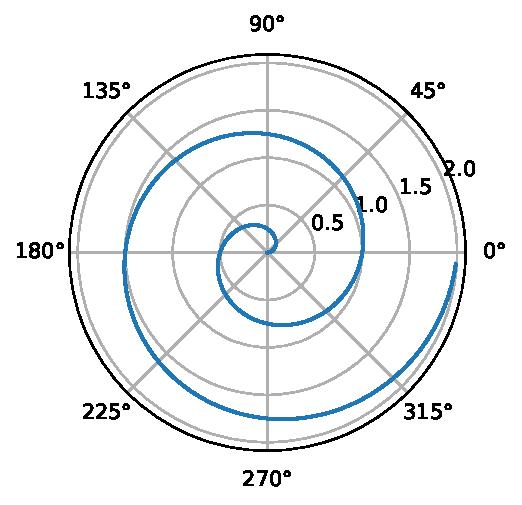
\includegraphics{proposal_files/figure-pdf/fig-polar-output-1.pdf}

}

\caption{\label{fig-polar}A line plot on a polar axis}

\end{figure}

Here's an example of citing a source (see Phillips 1999, 33--35). Be
sure the source information is entered in ``BibTeX'' form in the
\texttt{references.bib} file.

\hypertarget{references}{%
\section{References}\label{references}}

{[}The bibliography will automatically get generated. Any sources you
cite in the document will be included. Other entries in the
\texttt{.bib} file will not be included.{]}

test 1 2 3 4 5 6

\hypertarget{refs}{}
\begin{CSLReferences}{1}{0}
\leavevmode\vadjust pre{\hypertarget{ref-phil99}{}}%
Phillips, T. P. 1999. {``Possible Influence of the Magnetosphere on
{American} History.''} \emph{J. Oddball Res.} 98: 1000--1003.

\end{CSLReferences}



\end{document}
